
\begin{ex}%[0D7H2-1]
(2,0 điểm)
\begin{enumerate}
	\item Xét dấu của biểu thức $f(x)=3x^2-4x+1$.
	\item Giải bất phương trình $-x^2+3x-2 \geq 0$.
\end{enumerate}
\loigiai{
\begin{enumerate}
	\item Ta có $f(x)=0\Leftrightarrow 3x^2-4x+1=0 \Leftrightarrow \hoac{&x=1 \\ &x=\dfrac{1}{3}.}$\\
	Bảng xét dấu\\
	\centerline{
	
\begin{tikzpicture}[font=\footnotesize]
		\tkzTabInit
			{$x$/1, $f(x)$/0.7}
			{$-\infty$, $\dfrac{1}{3}$, $1$, $+\infty$}
		\tkzTabLine
			{, + , $0$ , - , $0$ , + ,}
	\end{tikzpicture}
	}\\
	Từ bảng xét dấu, kết luận
	\begin{itemize}
		\item $f(x)>0$ trên các khoảng $\left(-\infty;\dfrac{1}{3}\right)$, $(1;+\infty)$;
		\item $f(x)<0$ trên khoảng $\left(\dfrac{1}{3};1\right)$;
		\item $f(x)=0$ tại $x=\dfrac{1}{3}$, $x=1$.
	\end{itemize}
	\item Ta có $-x^2+3x-2=0 \Leftrightarrow \hoac{&x=1 \\ &x=2.}$\\
	Bảng xét dấu\\
	\centerline{
	\begin{tikzpicture}[font=\footnotesize]
		\tkzTabInit[lgt=3]
			{$x$/0.7, $-x^2+3x-2$/0.7}
			{$-\infty$, $1$, $2$, $+\infty$}
		\tkzTabLine
			{, - , $0$ , + , $0$ , - ,}
	\end{tikzpicture}
	}\\
	Từ bảng xét dấu ta có $-x^2+3x-2\geq 0 \Leftrightarrow 1 \leq x \leq 2$.\\
	Vậy tập nghiệm của bất phương trình là $S=[1;2]$.
\end{enumerate}
}
\end{ex}

\begin{ex}%[0D7H2-6]
(1,0 điểm) 
Tìm $m$ để bất phương trình $x^2-12mx-13 \geq 0$ nghiệm đúng với mọi $x$ thuộc $\mathbb{R}$.
\loigiai{
Ta có $\Delta'=(-6m)^2-1\cdot (-13)=36m^2+13>0$, $\forall m\in \mathbb{R}$.\\
Do đó phương trình $x^2-12mx-13=0$ luôn có hai nghiệm phân biệt.\\
Vậy không có giá trị $m$ nào để bất phương trình $x^2-12mx-13 \geq 0$ nghiệm đúng với mọi $x$ thuộc $\mathbb{R}$.
}
\end{ex}

\begin{ex}%[0D7N3-2]
(2,0 điểm)
Giải phương trình
\begin{enumerate}
	\item $\sqrt{x^2-6x-4}=\sqrt{x-4}$.
	\item $\sqrt{x^2-6x+6}=2x-1$.
\end{enumerate}
\loigiai{
\begin{enumerate}
	\item Điều kiện $x-4\geq 0 \Leftrightarrow x\geq 4$.\\
	Phương trình trở thành
	\begin{eqnarray*}
		&& x^2-6x-4 = x-4 \\
		&\Leftrightarrow& x^2-7x=0 \\
		&\Leftrightarrow& \hoac{&x=0 \\ &x=7.}
	\end{eqnarray*}
	Kết hợp với điều kiện, phương trình có nghiệm là $x=7$.
	\item Điều kiện $2x-1\geq 0 \Leftrightarrow x\geq \dfrac{1}{2}$.\\
	Phương trình trở thành
	\begin{eqnarray*}
		&& x^2-6x+6=(2x-1)^2 \\
		&\Leftrightarrow& x^2-6x+6 = 4x^2-4x+1 \\
		&\Leftrightarrow& 3x^2+2x-5 = 0\\
		&\Leftrightarrow& \hoac{&x=1 \\ &x=-\dfrac{5}{3}.}
	\end{eqnarray*}
	Kết hợp với điều kiện, phương trình có nghiệm $x=1$.
\end{enumerate}
}
\end{ex}
%Câu 4...........................
\begin{ex}%[0D7C3-6]%[Dự án đề kiểm tra Toán 10 GHKI NH23-24-Nguyễn Quang Hiệp]%[Bình Tân - TP HCM]
	(1,0 điểm)
	Hằng ngày bạn Hùng đều đón bạn Minh đi học tại một vị trí trên lề đường thẳng đến trường. Minh đứng tại vị trí $A$ cách lề đường một khoảng $50$ m để chờ Hùng. Khi nhìn thấy Hùng đạp xe đến địa điểm $B$, cách mình một đoạn $200$ m thì Minh bắt đầu đi bộ ra lề đường để bắt kịp xe. Vận tốc đi bộ của Minh là $5$ km/h, vận tốc xe đạp của Hùng là $15$ km/h. Hãy xác định vị trí $C$ trên lề đường (H.6.22) để hai bạn gặp nhau mà không bạn nào phải chờ người kia. (làm tròn kết quả đến hàng phần mười).
	\begin{center}
		\begin{tabular}{c}
			\begin{tikzpicture}[>=stealth,line join=round,line cap=round,font=\footnotesize,scale=1]
				\path[draw] 
				(0,0)coordinate (B)node[below]{$B$}node[above]{Hùng $\longrightarrow$}--++(0:6)coordinate (C)node[above]{$C$}--++(0:2)
				coordinate (H)node[above]{$H$}--++(-90:2)coordinate (A)node[below right]{$A$}node[below left]{Minh}node[midway,right]{$50$ m}--(C)node[midway,sloped,above]{$\mathbf{\longleftarrow}$}  (A)--(B)node[midway,below]{$200$ m}
				pic[draw,angle radius=2mm]{right angle=C--H--A};
				\draw[shorten <=-1cm,shorten >=-1cm,thick](B)--(H);	
			\end{tikzpicture}	\\
			Hình 6.22\\
		\end{tabular}
	\end{center}
	
	\loigiai{
		Đổi $200$ m$=0{,}2$ km, $50$ m=$0{,}05$ km.\\
		Đặt $CH=x$ (km) $(x>0)$.\\
		Xét tam giác $CHA$ vuông tại $H$, theo định lí Pythagore ta có
		\allowdisplaybreaks
		\begin{eqnarray*}
			C A^2=HA^2+HC^2=(0{,}05)^2+x^2=0{,}0025+x^2.
		\end{eqnarray*}
		Suy ra $CA=\sqrt{0{,}0025+x^2}$ hay quãng đường di chuyển của Minh từ vị trí $A$ đến điểm gặp nhau $C$ dài $\sqrt{0{,}0025+x^2}$ (km).\\
		Vận tốc đi bộ của Minh là $5$ km/h nên thời gian di chuyển của Minh từ vị trí $A$ đến điểm gặp nhau $C$ là $\dfrac{\sqrt{0{,}0025+x^2}}{5}$ (giờ).\\
		Xét tam giác $HAB$ vuông tại $H$, theo định lí Pythagore ta có
		\allowdisplaybreaks
		\begin{eqnarray*}
			A B^2=H B^2+H A^2 \Leftrightarrow H B^2=A B^2-H A^2=(0{,}2)^2-(0{,}05)^2=0{,}0375.
		\end{eqnarray*}
		Suy ra $HB=\dfrac{\sqrt{15}}{20}$.\\
		Ta có $BC+CH=HB \Leftrightarrow BC=HB-CH=\dfrac{\sqrt{15}}{20}-x$.\\
		Do đó quãng đường di chuyển của Hùng từ $B$ đến điểm gặp nhau $C$ dài $\dfrac{\sqrt{15}}{20}-x$ (km).\\
		Vận tốc đạp xe của Hùng là $15$ km/h nên thời gian di chuyển của Hùng từ $B$ đến điểm gặp nhau là $\dfrac{\dfrac{\sqrt{15}}{20}-x}{15}=\dfrac{\sqrt{15}-20 x}{300}$ (giờ).\\
		Để hai bạn gặp nhau mà không bạn nào phải chờ người kia thì thời gian di chuyển từ vị trí $A$ đến $C$ của Minh phải bằng thời gian di chuyển từ vị trí $B$ đến $C$ của Hùng.\\
		Khi đó ta có phương trình
		\allowdisplaybreaks
		\begin{eqnarray*}
			&&\dfrac{\sqrt{0{,}0025+x^2}}{5}=\dfrac{\sqrt{15}-20x}{300}\\
			&\Leftrightarrow &60 \sqrt{0{,}0025+x^2}=\sqrt{15}-20 x\\
			&\Leftrightarrow & 3600 \cdot\left(0{,}0025+x^2\right)=15-40 \sqrt{15} x+400 x^2 \\
			& \Leftrightarrow& 3200 x^2+40 \sqrt{15} x-6=0 \\
			& \Leftrightarrow& \heva{&x=\dfrac{-\sqrt{15}-3 \sqrt{7}}{160}\\&x=\dfrac{-\sqrt{15}+3 \sqrt{7}}{160}.}
		\end{eqnarray*}
		Lại có điều kiện của $x$ là $x>0$ nên ta chọn $x=\dfrac{-\sqrt{15}+3 \sqrt{7}}{160} \approx 0{,}0254$.\\
		Suy ra $B C=B H-C H \approx \dfrac{\sqrt{15}}{20}-0{,}0254 \approx 0{,}1682 ~km=168{,}2$ m.\\
		Vậy vị trí $C$ thỏa mãn yêu cầu đề bài là điểm cách $B$ khoảng $168{,}2$ m.
	}
\end{ex}

% Câu 5 
\begin{ex}%[0H9N4-2]%[Dự án đề kiểm tra Toán 10 GHKI NH23-24-Nguyễn Quang Hiệp]%[Bình Tân - TP HCM]
	(3,0 điểm)
	Trong mặt phẳng $O x y$, cho $\triangle A B C$ có $A(1; 2), B(-1; 1), C(-2; 3)$.
	\begin{enumerate}
		\item Tìm toạ độ trọng tâm tam giác $ABC$.
		\item Viết phương trình đường thẳng chứa cạnh $A B$ của $\triangle A B C$.
		\item Viết phương trình đường tròn tâm $A$ và đi qua điểm $B$.		
	\end{enumerate}
	\loigiai{
		\begin{enumerate}
			\item Gọi $G(x_G;y_G)$ là trọng tâm của tam giác $ABC$. khi đó
			\allowdisplaybreaks
			\begin{eqnarray*}
				\heva{&x_G=\dfrac{1+(-1)+(-2)}{3}=0\\&y_G=\dfrac{2+1+3}{3}=2.}
			\end{eqnarray*}		
			Vậy $\triangle ABC$ có trọng tâm là $G(0;2)$.
			\item Ta có $\overrightarrow{AB}=(2;1)$, khi đó véc-tơ pháp tuyến của đường thẳng $AB$ là $\overrightarrow{n}_{AB}=(1;-2)$.\\
			Phương trình của đường thẳng chứa cạnh $AB$ của $\triangle ABC$ là
			\allowdisplaybreaks
			\begin{eqnarray*}
				1\cdot (x-1)+(-2)\cdot (y-2)=0\Leftrightarrow x-2y+3=0.
			\end{eqnarray*}
			\item Ta có $AB=\sqrt{2^2+1^2}=\sqrt{5}$.\\
			Phương trình đường tròn tâm $A$ đi qua điểm $B$ là
			\allowdisplaybreaks
			\begin{eqnarray*}
				(x-1)^2+(y-2)^2=5.
			\end{eqnarray*}
		\end{enumerate}
	}
\end{ex}
%--------------------------------------

% Câu 6
\begin{ex}%[0H9H4-2%[Dự án đề kiểm tra Toán 10 GHKI NH23-24-Nguyễn Quang Hiệp]%[Bình Tân - TP HCM]
	(l,0 điểm)
	Trong hệ trục $Oxy$, cho $A(2;-1)$; $B(0; 5)$; $C(-3; 7)$. Tìm tọa độ tâm đường tròn ngoại tiếp tam giác $ABC$.		
	\loigiai{
		Gọi $(C):x^2+y^2-2ax-2by+c=0$ là phương trình đường tròn ngoại tiếp $\triangle ABC$. Khi đó ta có hệ phương trình
		\allowdisplaybreaks
		\begin{eqnarray*}
			\heva{&2^2+(-1)^2-2a\cdot 2-2b\cdot (-1)+c=0\\&0^2+5^2-2a\cdot 0-2b\cdot 5+c=0\\&(-3)^2+7^2-2a\cdot (-3)-2b\cdot 7+c=0}
			\Leftrightarrow \heva{&-4a+2b+c=-5\\&-10b+c=-25\\&6a-14b+c=-58}
			\Leftrightarrow \heva{&a=\dfrac{79}{14}\\&b=\dfrac{-3}{14}\\&c=-\dfrac{190}{7}.}
		\end{eqnarray*}	
		Vậy đường tròn ngoại tiếp tam giác $ABC$ có tâm là $I\left(\dfrac{79}{14};\dfrac{-3}{14}\right)$.
	}
\end{ex}
%--------------------------------------